\chapter{Strategie}
\label{chap:strategie}

\begin{center}
	\textit{"Better toilets for a better Future. "}
\end{center}

\section{Unternehmung}
\label{sec:unternehmung}

Unsere Mission ist es mit Smoilet 2.0 die ordin�re Toilette an das Internet of Things anzuschliessen. Die Unternehmung wurde am 1. April 2016 von sechs Studenten, der Fachrichtung Informatik ins Leben gerufen. Gem�ss unseres Leitbildes setzen wir stark auf Nachhaltigkeit in allen Aspekten.

\begin{figure}[H]
	\centering
	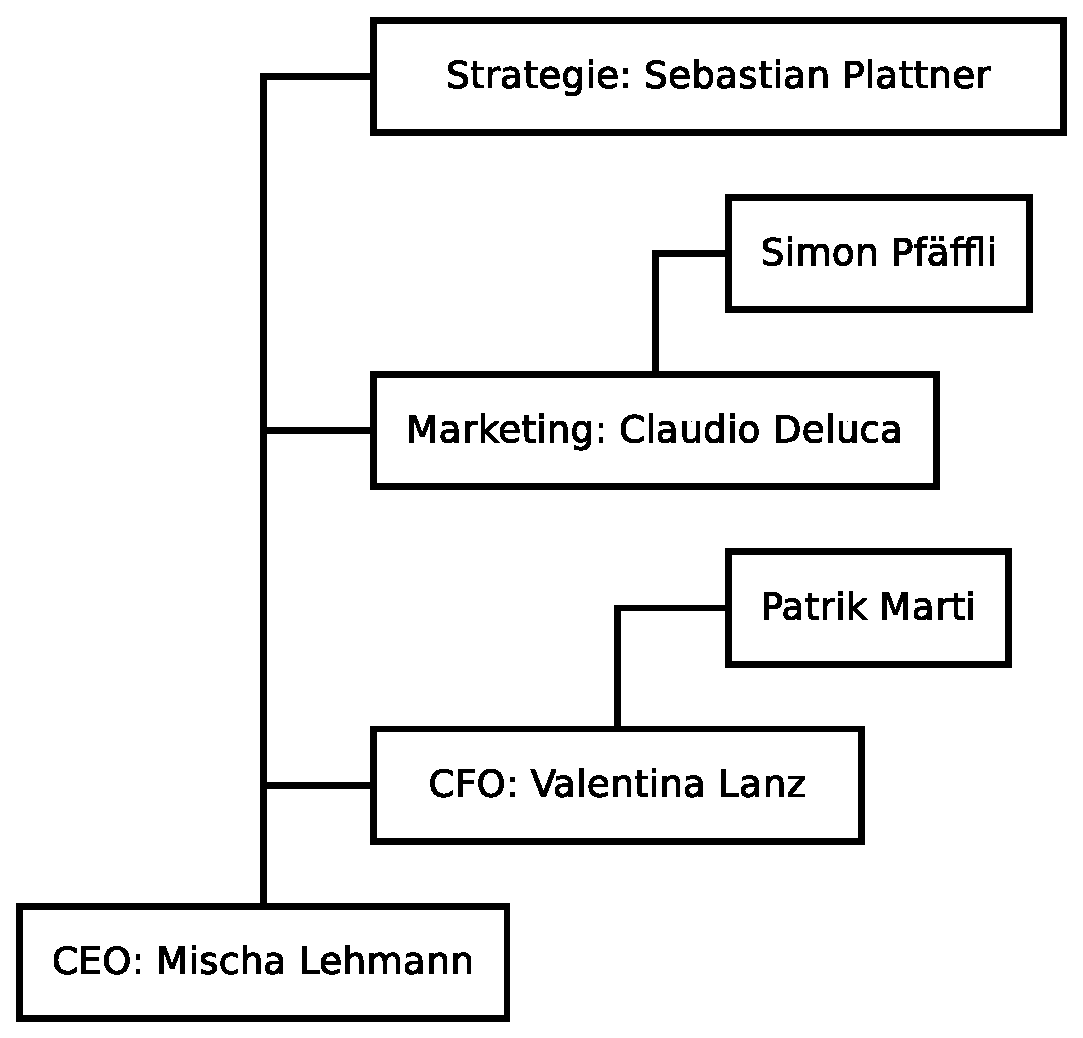
\includegraphics[scale=0.5]{bilder/organisation}
	\caption{Organigramm}
	\label{fig:organigramm}
\end{figure}

\section{Umgebungsanalyse}
\begin{center}
\begin{tabular}{ | l | l | l | } \hline
& Helpful & Harmful \\ \hline

% Internal view
\multirow{6}{*}{
\begin{sideways}
internal view
\end{sideways}}

% Internal view content
& \textbf{Strength (St�rken):} & \textbf{Weaknesses (Schw�chen):} \\ 
& ~~\llap{\textbullet}~ \underline{Einzigartigkeit}: Es werden keine �hnlichen & ~~\llap{\textbullet}~ \underline{Hohe Lohnkosten} \\
& Gadgets angeboten. & ~~\llap{\textbullet}~ \underline{Kein Eigenkapital}: Das gesamte Kapital wird \\
& ~~\llap{\textbullet}~ \underline{Starkes Management}: Wir haben ein Team & durch externe Investoren beschafft. \\
& zusammengestellt, welches in allen Gesch�fts- & ~~\llap{\textbullet}~ \underline{Erfahrung:} Wenig Erfahrung im Toiletten-Gesch�ft. \\
& bereichen gut ausgebildet ist. & \\ \hline

% External view
\multirow{8}{*}{
\begin{sideways}
external view
\end{sideways}}

% External view content
& \textbf{Opportunities (Chancen):} & \textbf{Threats (Gefahren):} \\
& ~~\llap{\textbullet}~ \underline{Marktpotenzial:} Es ist ein grosses Marktpotenzial  & ~~\llap{\textbullet}~ \underline{Produktstart:} Ein schlechter Produktstart oder \\ 
& vorhanden. Toiletten sind �berall zu finden. & Produktqualit�t k�nnte weitere Kunden vom Kauf \\
& ~~\llap{\textbullet}~ \underline{Markwachstum}: Starkes Marktwachstum Asien. & unseres Produktes abhalten. \\
&  & ~~\llap{\textbullet}~ \underline{Produktnachahmer}: M�gliche Konkurrenten k�nnten  \\
&  & bei Erfolg unseres Produktes in den Markt dr�ngen. \\
&  & ~~\llap{\textbullet}~ \underline{Ruf}: Neue Kunden werden nur Interesse an unserem \\ 
&  & Produkt zeigen, wenn wir einen guten Ruf haben. \\ \hline
\end{tabular}
\end{center}

\section{Marktanalyse}

5 Forces

\begin{landscape}
\section{Selbstanalyse}

\begin{center}
\begin{tabular}{ | l | l | l | } \hline

% empty
	& \textbf{Opportunities (Chancen)} 
	& \textbf{Threats (Gefahren)} \\
% empty
	& ~~\llap{\textbullet}~  \underline{Marktpotenzial}: Es ist ein grosses Marktpotenzial
	& ~~\llap{\textbullet}~  \underline{Produktstart}: Ein schlechter Produktstart oder \\
% empty
	& vorhanden. Toiletten sind �berall zu finden.
	& Produktqualit�t k�nnte weitere Kunden vom Kauf \\
% empty
	& ~~\llap{\textbullet}~ \underline{Markwachstum}: Starkes Marktwachstum in Asien.% empty
	& unseres Produktes abhalten. \\
% empty
	& % empty
	& ~~\llap{\textbullet}~ \underline{Produktnachahmer}: M�gliche Konkurrenten k�nnten \\
% empty
	& % empty
	& bei Erfolg unseres Produktes in den Markt dr�ngen. \\
% empty
	& % empty
	& ~~\llap{\textbullet}~ \underline{Ruf}: Neue Kunden werden nur Interesse an unserem \\
% empty
	& % empty
	& Produkt zeigen, wenn wir einen guten Ruf haben. \\
\hline 

% Strengths
\textbf{Strength (St�rken)}
	& \textbf{SO}-Massnahmen: 
	& \textbf{ST}-Massnahmen: \\
~~\llap{\textbullet}~ \underline{Einzigartigkeit}: Es werden keine �hnlichen
	& ~~\llap{\textbullet}~ Durch unser kleines und dynamisches Team k�nnen 
	& ~~\llap{\textbullet}~ Verst�rkung des PR-Teams zur Sicherstellung \\
Gadgets angeboten.
	& wir den Markt kreativ bearbeiten.
	& eines erfolgreichen Produkt-Releases. \\
 ~~\llap{\textbullet}~ \underline{Starkes Management}: Wir haben ein Team 
	&
	& ~~\llap{\textbullet}~ Aufbau eine Customer-Relation Team. \\
zusammengestellt, welches in allen Gesch�fts-
	&
	& \\
bereichen gut ausgebildet ist.
	&
	& \\	
\hline 

% Weaknesses
\textbf{Weaknesses (Schw�chen)}
	& \textbf{WO}-Massnahmen:
	& \textbf{WT}-Massnahmen:\\
~~\llap{\textbullet}~ \underline{Hohe Lohnkosten}
	& ~~\llap{\textbullet}~ Unsere Investoren sind mit den Playern im Markt
	& ~~\llap{\textbullet}~ Investorensuche zur Eigenkapitalst�rkung. \\
~~\llap{\textbullet}~ \underline{Kein Eigenkapital}: Das gesamte Kapital wird
	&  gut verkn�pft, so dass wir das Markt-Potential
	& ~~\llap{\textbullet}~ Kooperation. \\
durch externe Investoren beschafft.
	& optimal aussch�pfen k�nnen.
	& \\
~~\llap{\textbullet}~ \underline{Erfahrung}: Wenig Erfahrung im Toiletten-Gesch�ft
	&
	& \\
\hline

\end{tabular}
\end{center}

\end{landscape}